% Template for ICIP-2013 paper; to be used with:
%          spconf.sty  - ICASSP/ICIP LaTeX style file, and
%          IEEEbib.bst - IEEE bibliography style file.
% --------------------------------------------------------------------------
\documentclass{article}
\usepackage{spconf,amsmath,graphicx}
\usepackage[frenchb]{babel}
\usepackage[utf8]{inputenc}
\usepackage{graphicx}

% Example definitions.
% --------------------
\def\x{{\mathbf x}}
\def\L{{\cal L}}

% Title.
% ------
\title{D\'{E}CONVOLUTION D'IMAGES FLOUES PAR FILTRAGE CLS}
%
% Single address.
% ---------------
%\name{Author(s) Name(s)\thanks{Thanks to XYZ agency for funding.}}
%\address{Author Affiliation(s)}
%


\name{\qquad Julien Guichon \qquad Dimitri Gominski \qquad \qquad}

\address{}
	
\begin{document}
%\ninept
%
\maketitle
%
\begin{abstract}
	
	Image deblurring is a famous inverse problem in image processing, and can be frustrating because of the lack of information to retrieve the original image, often noisy and/or blurred with complex camera motion. It implies that the solution has to make assumptions on the acquisition system or the original image, and has to be robust against the heavy impact noise can have through the treatment.
	
	This reports study the performance and the limitations of the Constrained Least Squares (CLS ) approach. We also compare it to other famous algorithm, in order to determine under which conditions it should be use.
	
\end{abstract}
%

%
\section{Introduction}
\label{sec:intro}

	Le traitement de défloutage revient en termes mathématiques à effectuer une déconvolution sur l'image floutée. En effet, si $f(x,y)$ désigne l'image d'entrée, un "floutage" linéaire et indépendant de la position est modélisé par une opération de convolution par un noyau $h(x,y)$ qui donne l'image floutée $g(x,y)$ :
	$$g(x,y) = f(x,y) \otimes h(x,y)$$ 
	
	Dans ce cas, l'opération rigoureusement inverse de la convolution (déconvolution), correspondant à la résolution d'un système d'équations, suffit à retrouver exactement l'image de départ.
	
	Mais l'image d'entrée présentant systématiquement un bruit dû à l'acquisition, et les traitements numériques étant intrinsèquement sources de bruit, nous devons considérer un bruit additif n(x,y) : 
	$$g(x,y) = f(x,y) \otimes h(x,y) + n(x,y)$$ 
	
	Et c'est ce bruit qui complique grandement les calculs, puisque l'opération de déconvolution va l'amplifier au point de rendre l'image de sortie complètement inutilisable [2].
	
	Pour simplifier les notations et calculs, passons en calcul matriciel dans le domaine fréquentiel : 
	$$G = F * H + N$$
	
	Il existe 2 familles d'algorithmes de défloutage : les algorithmes qui supposent le noyau de floutage connu ($H$), et les algorithmes "à l'aveugle" où aucune supposition n'est faite sur le processus de floutage.
	
	

\section{Floutages usuels}
\label{sec:format}

	Le floutage peut être dû : 
	\begin{itemize}
	\item à des mouvements intempestifs du système d'acquisition ou de l'objet lors de la prise
	\item à des perturbations optiques lors du passage des rayons lumineux dans certains milieux (verre, eau)
	\item à une modification de la distance focale pendant la prise (zoom/dézoom, parfois voulu)
	\end{itemize}

	On caractérise ce floutage par un noyau $h(x,y)$. Cette fonction qu'on appelle PSF (\textit{Point Spread Function}) donne la réponse d'un théorique "système de floutage" (système qui donnerait l'image de sortie floutée à partir de l'image d'entrée) à une entrée correspondant à un point lumineux au centre de l'image (impulsion lumineuse). Son équivalent fréquentiel est appelé OTF (\textit{Optical Transfer Function}). Ci-dessous deux exemples de noyaux usuels :
	
	\begin{figure}[h]
		\begin{center}			
			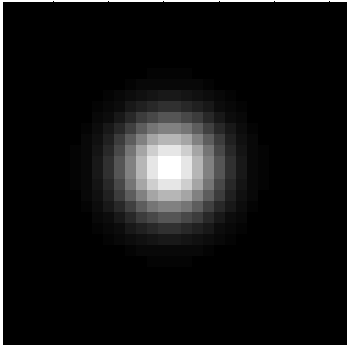
\includegraphics[scale=0.3]{Img/blurkernel_gauss}
		\end{center}
		\caption{Noyau de floutage gaussien}
	\end{figure}

	
	\begin{figure}[h]
	\begin{center}			
		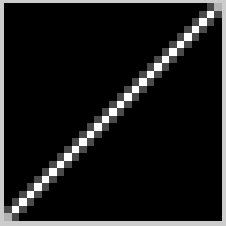
\includegraphics[scale=0.48]{Img/blurkernel_linear}
	\end{center}
	\caption{Noyau de floutage linéaire}
	\end{figure}

	Le noyau linéaire correspond par exemple à un mouvement linéaire de l'appareil pendant la prise, et le noyau gaussien à une capture à travers du verre (diffusion).
	Ces exemples étant très courants, nous ferons notre étude de l'algorithme CLS sur ces deux noyaux.
	

\section{Approches classiques - bibliographie}
\label{sec:pagestyle}

	Plusieurs méthodes ont été proposées pour trouver une estimation correcte $\hat f$ de l'image d'origine $f$ à partir de la sortie $g$, en supposant le noyau de floutage $h$ connu.
	
	De manière générale, l'idée pour pouvoir effectuer une déconvolution en limitant les effets du bruit est de le filtrer aux fréquences concernées. Aux fréquences non impactées par le bruit, l'opération dans le domaine fréquentiel doit idéalement être une inversion, en effet si $N(f_1,f_2) = 0$, on a $G(f_1,f_2) = \hat F(f_1,f_2) * H(f_1,f_2)$ donc :
	$$\hat F(f_1,f_2) = G(f_1,f_2) * H^{-1}(f_1,f_2)$$
	
	Application du filtre de Wiener qui fait usage de la répartition spectrale du signal et du bruit supposées connues, la déconvolution de Wiener [4] propose une estimation $\hat F$ comme suit :
	$$\hat F = \frac {1}{H} \bigg[ \frac {|H|^2}{|H|^2 + \frac {|N|^2}{|F|^2} } \bigg] * G$$
	
	On voit que le filtre appliqué à G est lié à l'évolution du rapport signal/bruit $\frac{|F|^2}{|N|^2}$ dans le domaine fréquentiel, de manière à ce que les fréquences polluées ($\frac{1}{SNR} { \rightarrow +\infty}$) soient éliminées avec l'augmentation du dénominateur, tandis qu'aux fréquences non polluées ($\frac{1}{SNR} { \rightarrow 0}$) on fasse rigoureusement une inversion de $H$.
	
	Cette opération revient à minimiser l'erreur quadratique moyenne entre l'image d'entrée et son estimation, son défaut est de faire des hypothèses fortes sur le bruit et l'image d'entrée qui ne sont pas toujours disponibles.
	\\
	
	Les papiers [5] et [6] proposent de décomposer la matrice $H$, de manière à fournir des coefficients caractéristiques sur lesquels on peut agir pour réduire les effets du bruit, notamment avec la décomposition SVD qui fournit la décomposition suivante d'une matrice M :
	$$ M = U \Sigma V^*$$
	
	Avec $\Sigma$ matrice diagonale des coefficients. Une telle décomposition facilite la résolution du problème inverse du floutage, mais se révèle très conséquent en temps de calcul.
	
	Des approches statistiques [7] ont également été essayées, où une première estimation du noyau de floutage est donnée puis affinée au cours de plusieurs itérations. 
	
	
\section{TYPE-STYLE AND FONTS}
\label{sec:typestyle}

To achieve the best rendering both in printed proceedings and electronic proceedings, we
strongly encourage you to use Times-Roman font.  In addition, this will give
the proceedings a more uniform look.  Use a font that is no smaller than nine
point type throughout the paper, including figure captions.

In nine point type font, capital letters are 2 mm high.  {\bf If you use the
smallest point size, there should be no more than 3.2 lines/cm (8 lines/inch)
vertically.}  This is a minimum spacing; 2.75 lines/cm (7 lines/inch) will make
the paper much more readable.  Larger type sizes require correspondingly larger
vertical spacing.  Please do not double-space your paper.  TrueType or
Postscript Type 1 fonts are preferred.

The first paragraph in each section should not be indented, but all the
following paragraphs within the section should be indented as these paragraphs
demonstrate.

\section{MAJOR HEADINGS}
\label{sec:majhead}

Major headings, for example, "1. Introduction", should appear in all capital
letters, bold face if possible, centered in the column, with one blank line
before, and one blank line after. Use a period (".") after the heading number,
not a colon.

\subsection{Subheadings}
\label{ssec:subhead}

Subheadings should appear in lower case (initial word capitalized) in
boldface.  They should start at the left margin on a separate line.
 
\subsubsection{Sub-subheadings}
\label{sssec:subsubhead}

Sub-subheadings, as in this paragraph, are discouraged. However, if you
must use them, they should appear in lower case (initial word
capitalized) and start at the left margin on a separate line, with paragraph
text beginning on the following line.  They should be in italics.

\section{PRINTING YOUR PAPER}
\label{sec:print}

Print your properly formatted text on high-quality, 8.5 x 11-inch white printer
paper. A4 paper is also acceptable, but please leave the extra 0.5 inch (12 mm)
empty at the BOTTOM of the page and follow the top and left margins as
specified.  If the last page of your paper is only partially filled, arrange
the columns so that they are evenly balanced if possible, rather than having
one long column.

In LaTeX, to start a new column (but not a new page) and help balance the
last-page column lengths, you can use the command ``$\backslash$pagebreak'' as
demonstrated on this page (see the LaTeX source below).

\section{PAGE NUMBERING}
\label{sec:page}

Please do {\bf not} paginate your paper.  Page numbers, session numbers, and
conference identification will be inserted when the paper is included in the
proceedings.

\section{ILLUSTRATIONS, GRAPHS, AND PHOTOGRAPHS}
\label{sec:illust}

Illustrations must appear within the designated margins.  They may span the two
columns.  If possible, position illustrations at the top of columns, rather
than in the middle or at the bottom.  Caption and number every illustration.
All halftone illustrations must be clear black and white prints.  Colors may be
used, but they should be selected so as to be readable when printed on a
black-only printer.

Since there are many ways, often incompatible, of including images (e.g., with
experimental results) in a LaTeX document, below is an example of how to do
this \cite{Lamp86}.

\section{FOOTNOTES}
\label{sec:foot}

Use footnotes sparingly (or not at all!) and place them at the bottom of the
column on the page on which they are referenced. Use Times 9-point type,
single-spaced. To help your readers, avoid using footnotes altogether and
include necessary peripheral observations in the text (within parentheses, if
you prefer, as in this sentence).

% Below is an example of how to insert images. Delete the ``\vspace'' line,
% uncomment the preceding line ``\centerline...'' and replace ``imageX.ps''
% with a suitable PostScript file name.
% -------------------------------------------------------------------------
\begin{figure}[htb]

\begin{minipage}[b]{1.0\linewidth}
  \centering
%  \vspace{2.0cm}
  \centerline{(a) Result 1}\medskip
\end{minipage}
%
\begin{minipage}[b]{.48\linewidth}
  \centering
%  \vspace{1.5cm}
  \centerline{(b) Results 3}\medskip
\end{minipage}
\hfill
\begin{minipage}[b]{0.48\linewidth}
  \centering
%  \vspace{1.5cm}
  \centerline{(c) Result 4}\medskip
\end{minipage}
%
\caption{Example of placing a figure with experimental results.}
\label{fig:res}
%
\end{figure}


% To start a new column (but not a new page) and help balance the last-page
% column length use \vfill\pagebreak.
% -------------------------------------------------------------------------
%\vfill
%\pagebreak

\section{COPYRIGHT FORMS}
\label{sec:copyright}

You must include your fully completed, signed IEEE copyright release form when
form when you submit your paper. We {\bf must} have this form before your paper
can be published in the proceedings.

\section{REFERENCES}
\label{sec:ref}

List and number all bibliographical references at the end of the
paper. The references can be numbered in alphabetic order or in
order of appearance in the document. When referring to them in
the text, type the corresponding reference number in square
brackets as shown at the end of this sentence \cite{C2}. An
additional final page (the fifth page, in most cases) is
allowed, but must contain only references to the prior
literature.

% References should be produced using the bibtex program from suitable
% BiBTeX files (here: strings, refs, manuals). The IEEEbib.bst bibliography
% style file from IEEE produces unsorted bibliography list.
% -------------------------------------------------------------------------
\bibliographystyle{IEEEbib}
\bibliography{strings,refs}

\end{document}
